%% =====================================================================================
%% 4 Self-play across risk, plus prompt and decoding controls.
%% Numbers: tables/num_selfplay.tex (analysis/selfplay.py). Figure: fig_selfplay.pdf.
%% Tables: tab_models.tex, tab_robust.tex (tabular only; captions live here).
%% =====================================================================================
\section{Risk does not change the default}
\label{sec:risk}

\begin{figure*}[t]
\centering
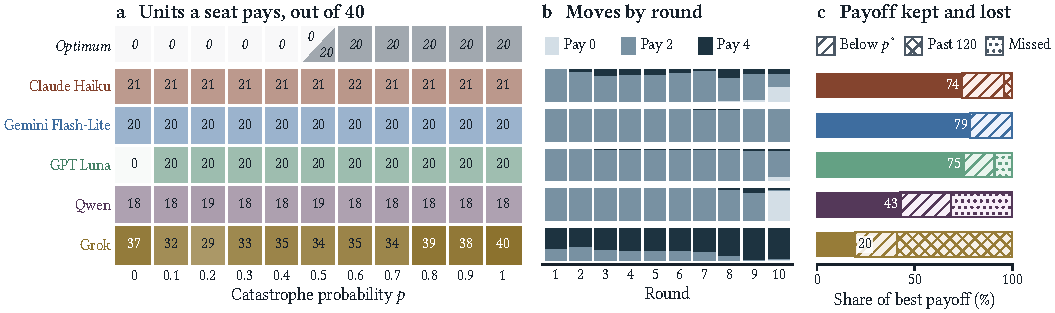
\includegraphics[width=\textwidth]{figures/fig_selfplay.pdf}
\Description{Three panels that share one row per model, below a reference row. Left: a grid
of the mean units a seat pays at each catastrophe probability from 0 to 1. The optimum row
switches from 0 to 20 at one half, while the model rows barely change: about 20 for four
models, 0 only for GPT Luna at probability zero, and 29 to 40 for Grok. Middle: for each round,
the share of seats paying 0, 2 or 4; Qwen pays 2 until round 10 and then almost always 0, and
Grok mostly pays 4. Right: bars of the share of the best attainable payoff each model keeps;
Grok keeps about a fifth and loses most by paying past the target, and Qwen loses most by
missing it.}
\caption{Self-play on the risk grid, 110 games per model. (a)~Mean units a seat pays out of
40, ten games per cell; the top row is the optimum of Proposition~\ref{prop:eq}, where both 0
and 20 are optimal at $p=0.5$. (b)~Share of seats paying 0, 2 or 4 in each round, over the
100 games with $p>0$. (c)~Expected payoff kept as a share of $\mathrm{opt}(p)$, and the loss
split into paying toward the target below $\popt$, paying past 120, and missing the target at
or above $\popt$.}
\label{fig:selfplay}
\end{figure*}

Four of the five models pay about the fair share at every positive risk level
(Figure~\ref{fig:selfplay}). For Claude Haiku, Gemini Flash-Lite, GPT Luna and Qwen, the mean
total below the pivot and the mean total above it differ by at most \GridStepMaxOther{}
units, while a risk-neutral player would jump from 0 to 20. Risk aversion does not explain
the flat line either: preferring a certain 20 to keeping 40 with probability 0.9 requires a
coefficient of relative risk aversion of at least \GridCrraLow{}. Gemini Flash-Lite is the
clearest case: \GridFlashExactPct\% of its seats play the exact split at every risk level, so
its play is optimal above the pivot only because a fixed rule matches the optimum there.

\paragraph{Paying when there is nothing to protect.}
\GridZeroModelsPayingCap{} of the five models pay at $p=0$, close to their usual amount,
although paying there only lowers a player's own money (\GridZeroPaying{} of
\GridZeroSeats{} seats pay). GPT Luna is the one exception: it pays nothing at $p=0$ and its
usual share at every positive risk, so it separates no risk from some risk but does not
grade the risk.

\paragraph{Three ways to lose.}
The models lose payoff in three ways (Table~\ref{tab:models}). Gemini Flash-Lite, Claude
Haiku and GPT Luna lose mostly below the pivot, where they pay for a target that is not worth
reaching. Grok pays far more than needed: its groups reach the target by round
\GridGrokSecuredRound{} on average, and each seat then pays another \GridGrokWaste{} units
into a pool that is already safe. Qwen fails at the end. It pays 2 in
\GridQwenRoundsOneNinePct\% of decisions in rounds 1 to 9 and then \GridQwenLastZeroPct\% of
its seats pay nothing in round 10, so its groups reach the target in only \GridQwenReach{} of
110 games; had each seat repeated its round-9 move, \GridQwenFixReachPct\% would have
succeeded. This is a coordination failure, not one bad move: with 108 in the pool before
round 10, one seat alone can add at most 4, so paying nothing is also an equilibrium of that
round, and Qwen seats almost always pick it, much as human contributions decline at the end
of repeated public goods games~\cite{andreoni1988free}. GPT Luna shows a milder form: its
groups miss the target in \GridLunaMiss{} of \GridLunaGames{} games with $p>0$, always after
keeping pace until the last round. Claude Haiku shows that the pool can be read from the same
prompt: it pays nothing in round 10 in \GridHaikuStopPct\% of seats once the pool has reached
the target, against \GridHaikuStopOtherPct\% when it has not. Success rates hide all of this.
Gemini Flash-Lite and Grok both reach the target in every game, yet Grok keeps a quarter as
much money, and the panel loses \GridLossPanelPct\% of the attainable payoff.

\begin{table}[t]
\caption{Self-play summary over the risk grid, using expected payoffs. \emph{Pays at
$p{=}0$} is the mean seat total where paying is dominated. \emph{Exact split} is the share of
seats paying 2 in all ten rounds. \emph{Target} is the share of games that reach it, and
\emph{Payoff} is the expected payoff per seat; the optimum averages \GridOptMean{} over the
grid. \emph{Lost} is the share of the attainable payoff $\mathrm{opt}(p)$ that was lost, and
\emph{Main loss} is its largest cause: paying toward the target below $\popt$, paying beyond
120, or missing the target at or above $\popt$, which for Qwen happens in the last round.}
\label{tab:models}
% Generated by paper/AAMAS/analysis/selfplay.py. Do not edit by hand.
\begin{tabular}{@{}l@{\hspace{3pt}}r@{\hspace{3pt}}r@{\hspace{3pt}}r@{\hspace{3pt}}r@{\hspace{3pt}}r@{\hspace{3pt}}l@{}}
\toprule
 & Pays at & Exact & Target & Payoff & Lost & Main \\
Model & $p{=}0$ & split (\%) & (\%) & & (\%) & loss \\
\midrule
Claude Haiku & 20.9 & 17 & 98 & 18.9 & 26 & below $p^*$ \\
Gemini Flash-Lite & 20.0 & 99.7 & 100 & 20.0 & 21 & below $p^*$ \\
GPT Luna & 0.0 & 72 & 70 & 19.2 & 25 & below $p^*$ \\
Qwen & 18.0 & 4 & 2 & 10.9 & 57 & last round \\
Grok & 37.4 & 2 & 100 & 5.0 & 80 & overshoot \\
\bottomrule
\end{tabular}

\end{table}

\paragraph{The default survives rewording, but its failures do not.}
Deleting the two equal-split phrases does not lower anyone's payment
(Table~\ref{tab:robust}), so the hint was a ceiling and a guide for precision, not the source
of the cooperation. Gemini Flash-Lite still plays the exact split, which it can rebuild from
the target, and GPT Luna keeps its average but not its precision (the exact split falls from
\NoCueLunaExactBasePct\% to \NoCueLunaExactPct\% of seats). Qwen and Grok pay more; Qwen now
reaches the target in \NoCueQwenReach\% of games instead of \NoCueQwenReachBase\%, but earns
less because it overpays. Two rewordings and a temperature of zero leave the mean payments of
the other four models within \RobFlatMaxShift{} unit of the grid. The failures are less stable
than the means: under the second rewording Grok pays the fair share, and the share of Qwen
seats that pay nothing in round 10 ranges from \RobQwenLastZeroNoHint\% to
\RobQwenLastZeroParaTwo\% across prompts. Grok's rise with risk on the grid
(\RobGrokRiskBase{} units) shrinks to \RobGrokRiskRerun{} in the rerun, so we do not read it
as a response to risk.

\paragraph{Stating the goal, not removing the norms, switches the default off.}
The default does not come from the normative words. With the neutral wording,
\WorZeroModelsPaying{} models still pay at $p=0$ (\WorZeroPaying{} of \WorZeroSeats{} seats
pay), and at $p=0.1$ and $p=0.9$ four models pay what they paid before while Grok pays even
more (Table~\ref{tab:robust}). Adding the stated goal changes play at zero risk: Claude Haiku,
Gemini Flash-Lite and Qwen then pay \NeuZeroHaiku{}, \NeuZeroFlashLite{} and \NeuZeroQwen{}
units at $p=0$, against \GridZeroHaiku{}, \GridZeroFlashLite{} and \GridZeroQwen{} with the
base prompt. The goal does not make most models weigh the risk. Claude Haiku and Gemini
Flash-Lite still pay the fair share at $p=0.1$ (\NeuLowHaiku{} and \NeuLowFlashLite{} units),
so they separate no risk from some risk but do not grade it. GPT Luna alone grades it, paying
\NeuLowLuna{} units at $p=0.1$ and \NeuHighLuna{} at $p=0.9$. Qwen pays less at every level
and reaches the target in \NeuReachQwen{} of \NeuGamesQwen{} games, and Grok keeps paying far
more than needed. The default is therefore what these models do when the prompt leaves their
goal unstated; the scripted and mixed designs below use the base prompt and describe it.

\begin{table}[t]
\caption{Mean seat total under prompt and decoding changes, pooled over $p=0.1$ and $0.9$
(20 games per entry). \emph{Base} is the self-play grid. \emph{Rerun} is the in-game
question condition, which uses the unchanged prompt and was collected with the other
changes. \emph{No hint} deletes the equal-split phrases, \emph{Para.\,1} and \emph{Para.\,2}
are the two rewordings, \emph{Temp.\,0} sets the temperature to zero, \emph{Wording} uses the
neutral wording, and \emph{Neutral} adds the stated goal to it. Bold marks a shift from
\emph{Base} of at least 2 units with permutation $P<0.01$. Temperature zero was not
deterministic: a cell produced \RobTempZeroDistinct{} distinct games in ten, against
\RobTempZeroBaseDistinct{} at 0.7.}
\label{tab:robust}
% Generated by paper/AAMAS/analysis/selfplay.py. Do not edit by hand.
\begin{tabular}{@{}lrrrrr@{}}
\toprule
 & Claude & Gemini & GPT &  &  \\
Condition & Haiku & Flash-Lite & Luna & Qwen & Grok \\
\midrule
Base & 20.9 & 20.0 & 19.9 & 18.4 & 35.1 \\
Rerun & 21.3 & 20.0 & 19.9 & 18.5 & 35.6 \\
No hint & 21.7 & 20.0 & 19.9 & \textbf{34.7} & \textbf{40.0} \\
Para.\,1 & 21.3 & 20.0 & 19.9 & 19.4 & 31.8 \\
Para.\,2 & 20.9 & 20.0 & 19.8 & 18.0 & \textbf{20.6} \\
Temp.\,0 & 21.2 & 20.0 & 20.0 & 18.3 & 35.1 \\
Wording & 21.0 & 20.0 & 19.4 & 18.7 & \textbf{39.7} \\
Neutral & 20.0 & 20.1 & \textbf{13.9} & \textbf{8.2} & 37.7 \\
\bottomrule
\end{tabular}

\end{table}
